%------------------------FIRST------------------------
%------------------------------------------------

\begin{frame}
	\frametitle{Содержание доклада}
	\begin{enumerate}
	\item Дуальная структура;\newline
	\item Прохождение критической энергии;\newline
	\item Исследование ЭДМ.
	\end{enumerate}
\end{frame}
%------------------------------------------------
\section{Дуальная структура}
%------------------------------------------------
\begin{frame}
	\centering \Large{Дуальная структура}
\end{frame}
%------------------------------------------------
\begin{frame}
	\frametitle{Дуальная структура}
	При разработке структуры, удовлетворяющей требованиям, предъявляемым к частицам с различным зарядом, важно создать перестраиваемую структуру без внесения конструктивных изменений. Мы назвали такую структуру -- \textit{дуальной}.
	\vspace{2em} 
	
	\begin{columns}
		\begin{column}{0.5\textwidth}
			\raggedright
			\adjustbox{valign=t}{\begin{minipage}[t]{\linewidth}
				\centering \textbf{Тяжёлые ионы}\\
				обладают более выраженным эффектом разогрева из-за внутрипучкового рассеяния.\\
			\end{minipage}}
		\end{column}
		\hfill
		\begin{column}{0.5\textwidth}
			\raggedright
			\adjustbox{valign=t}{\begin{minipage}[t]{\linewidth}
				\centering{\textbf{Лёгкие частицы}}\\
				влияние критической энергии на динамику сгустка.\\
			\end{minipage}}
		\end{column}
		\begin{column}{0.01\textwidth}
		\end{column}
	\end{columns}
	\vspace{2em}
\footnotetext[1]{(to be published) Kolokolchikov S.D., et al. Features of dual-purpose structure for heavy ion and light particles, Nucl.Sci. and Tech.}		
\end{frame}
%------------------------------------------------
\begin{frame}
	\frametitle{Регулярная структура}
	\begin{columns}
		\begin{column}{0.3\textwidth}
			\raggedright
			\adjustbox{valign=t}{\begin{minipage}[t]{\linewidth}
				В классической регулярной структуре $\gamma_{\text{tr}}\simeq\nu_{x}$. \\
				При одинаковой магнитной жесткости $B\rho$ максимальная энергия для легких частиц выше, чем для тяжелых ионов, из-за их соотношения заряд-масса.
			\end{minipage}}
		\end{column}
		\begin{column}{0.7\textwidth}
			\begin{minipage}{\linewidth}
				\centering
				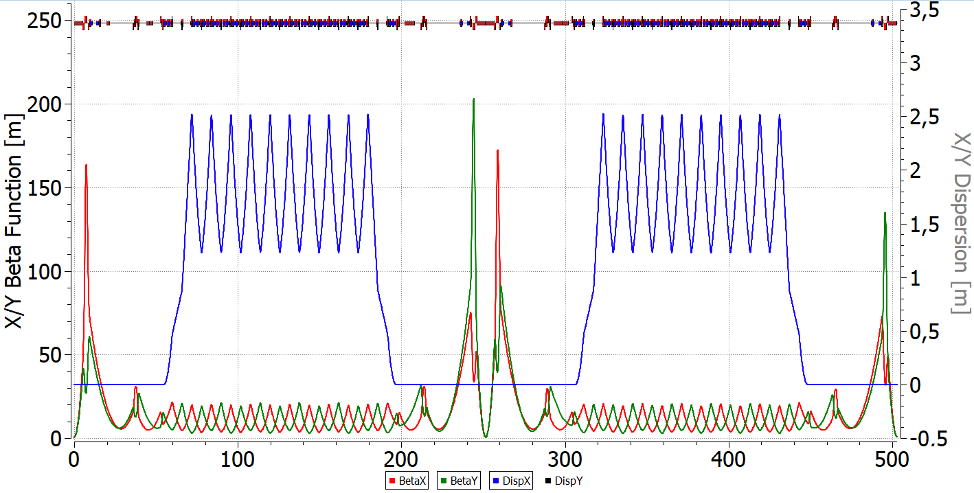
\includegraphics[width=1\linewidth]{images/1_regular}
			\end{minipage}
		\end{column}
	\end{columns}
\end{frame}
%------------------------------------------------
\begin{frame}
	\frametitle{Резонансная структура}
	\begin{columns}
	\begin{column}{0.3\textwidth}
		\raggedright
		\adjustbox{valign=t}{\begin{minipage}[t]{\linewidth}
		Может быть получена из регулярной структуры путем разделения фокусирующих квадруполей на 2 семейства с различными градиентами.		
		\end{minipage}}
	\end{column}
	\begin{column}{0.7\textwidth}
		\begin{minipage}{\linewidth}
			\centering
			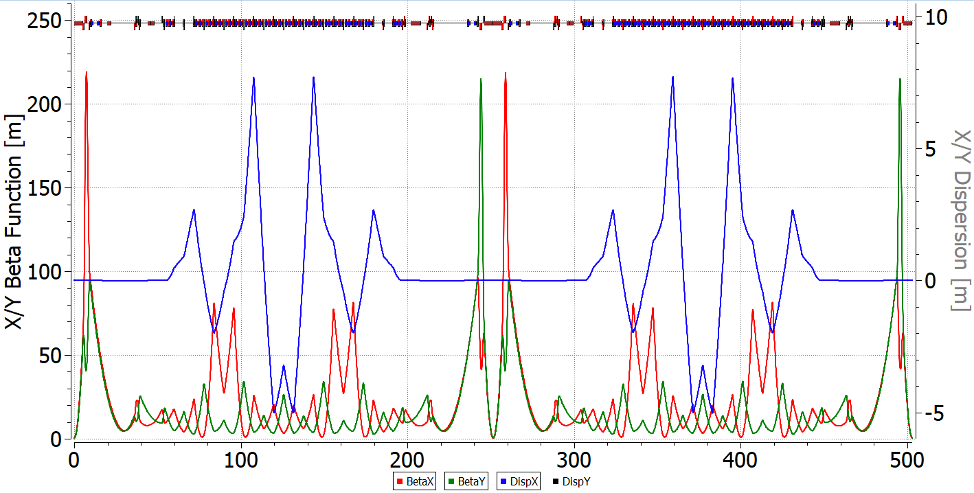
\includegraphics[width=1\linewidth]{images/1_resonant}
		\end{minipage}
	\end{column}
\end{columns}
\footnotetext[2]{Колокольчиков С.Д., Сеничев Ю.В. Магнито-оптическая Структура Коллайдера NICA c Высокой Критической Энергией. Яд. Физ. и Инж. том 13, номер 1, стр. 27-36 (2022). DOI: 10.56304/S2079562922010171}
\footnotetext[3]{Колокольчиков С.Д., Сеничев Ю.В. Особенности Прохождения и Повышения Критической Энергии Синхротрона. Яд. Физ. и Инж. том 14, номер 6, стр. 587-592 (2023).  DOI: 10.56304/S2079562923010153}
\end{frame}
%------------------------------------------------
\begin{frame}
	\frametitle{Комбинированная структура}
	\begin{columns}
		\begin{column}{0.3\textwidth}
			\raggedright
			\adjustbox{valign=t}{\begin{minipage}[t]{\linewidth}
					Реальная арка
					\begin{equation} \label{eq:eta_pk}
						\eta_{\textrm{pk}}=\frac{1}{\gamma_{\textrm{tr}}^2}-\frac{1}{\gamma^2}
					\end{equation}
					\noindent компенсируется аркой с комплексным значением критической энергии
					\begin{equation} \label{eq:eta_kp}
						\eta_{\textrm{kp}}=-\frac{1}{\gamma_{\textrm{tr}}^2}-\frac{1}{\gamma^2}\ \ \ 
					\end{equation}
			\end{minipage}}
		\end{column}
		\begin{column}{0.7\textwidth}
			\begin{minipage}{\linewidth}
				\centering
				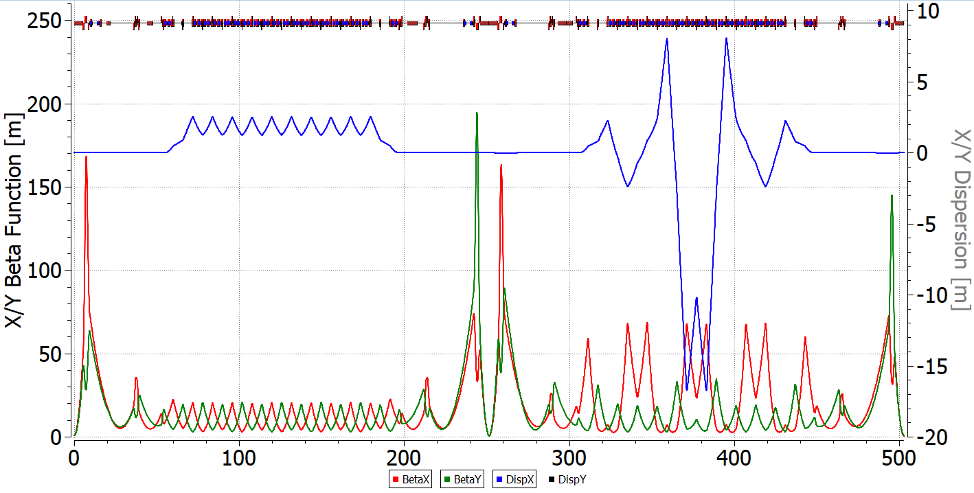
\includegraphics[width=1\linewidth]{images/1_combined}
			\end{minipage}
		\end{column}
	\end{columns}
\end{frame}
%------------------------------------------------
\begin{frame}
	\frametitle{Стохастическое охлаждение}
	\begin{equation}
		\frac{1}{\tau_{\text{tr,l}}}=A\cdot\frac{W}{N} \frac{\left(1-1 / {M_{\text{pk}}}^2\right)^2}{M_{\text{kp}}}; \quad
		M_{\text{pk}} =\frac{1}{2\left(f_{\max}+f_{\min}\right) \eta_{\textrm{pk}} T_{\textrm{pk}} \delta}; \quad 
		M_{\text{kp}} =\frac{1}{2\left(f_{\max}-f_{\min}\right) \eta_{\textrm{kp}} T_{\textrm{kp}} \delta}.
	\end{equation}

	\begin{columns}
		\begin{column}{0.5\textwidth}
			\raggedright
			\adjustbox{valign=t}{\begin{minipage}[t]{\linewidth}
				Асимптотический рост в двух случаях:
				\begin{enumerate}
					\item $\eta\rightarrow\frac{1}{2\left(f_{\text{max}}+f_{\text{min}}\right)T_{\text{pk}}\delta}$, Schottky-спектр пучка становится сплошным и $M_{\text{pk}}\rightarrow1$;
					\item $\eta\rightarrow0$, перемешивание на пути от киккера к пикапу не происходит и $M_{\text{kp}}\rightarrow\infty$.
				\end{enumerate}
			\end{minipage}}
		\end{column}
		\begin{column}{0.5\textwidth}
			\begin{minipage}{\linewidth}
				\centering
				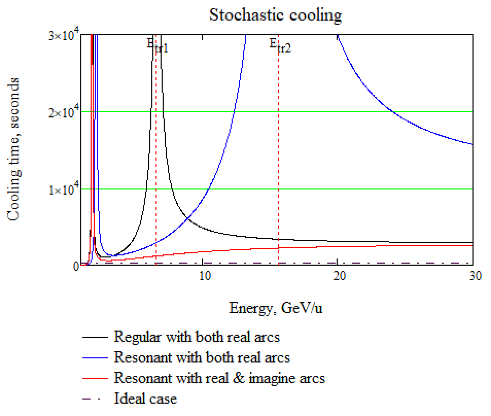
\includegraphics[width=0.7\linewidth]{images/1_SC_wide}
			\end{minipage}
		\end{column}
	\end{columns}
\end{frame}
%------------------------------------------------
\begin{frame}
	\frametitle{Внутрипучковое рассеяние}
	\begin{equation}
		\frac{1}{\tau_x}=\frac{\pi^2r_0^2v_cm^3N\left(log\right)}{\gamma\Gamma}\left[\frac{\gamma^2\left(D_x^2+\beta_x^2\phi_x^2\right)}{\epsilon_x\beta_x}\right]\int_{0}^{\infty}\frac{d\lambda\ \lambda^\frac{1}{2}\left[a_x\lambda+b_x\right]}{\left(\lambda^3+a\lambda^2+b\lambda+c\right)^\frac{3}{2}}
		\label{eq:IBS}
	\end{equation}
	
	\begin{columns}
		\begin{column}{0.4\textwidth}
			\raggedright
			\adjustbox{valign=t}{\begin{minipage}[t]{\linewidth}
					Из сравнения времени внутрипучкового рассеяния со временем охлаждения можно сделать заключение, что в регулярной структуре стохастическое охлаждение способно сбалансировать внутрипучковое рассеяние в диапазоне энергий $W\geq4.5$ ГэВ/нуклон.
			\end{minipage}}
		\end{column}
		\begin{column}{0.6\textwidth}
			\begin{minipage}{\linewidth}
				\centering
				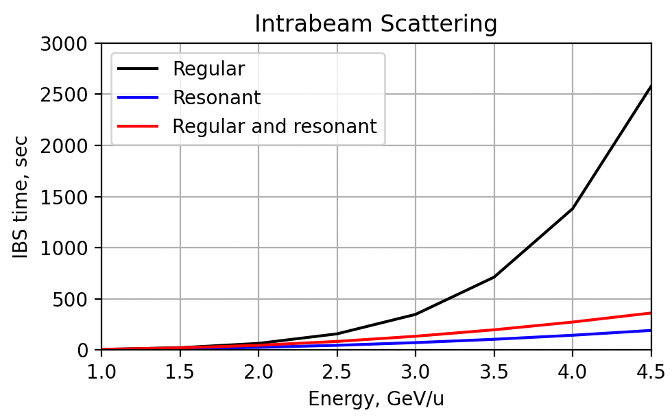
\includegraphics[width=0.8\linewidth]{images/1_IBS}
			\end{minipage}
		\end{column}
	\end{columns}
\end{frame}
%------------------------------------------------
%------------------------SECOND------------------------
%------------------------------------------------
\section{Прохождение критической энергии}
%------------------------------------------------
\begin{frame}
	\centering \Large{Прохождение критической энергии}
\end{frame}
%------------------------------------------------
\begin{frame}
	\frametitle{Скачок критической энергии в У-70}
	
	\begin{columns}
		\begin{column}{0.4\textwidth}
			\raggedright
			\adjustbox{valign=t}{\begin{minipage}[t]{\linewidth}
				Вспомогательные квадруполи расположены через полпериода $\Delta\nu_{x,y}=0.5\times0.5$ и имеют противоположные полярности.
				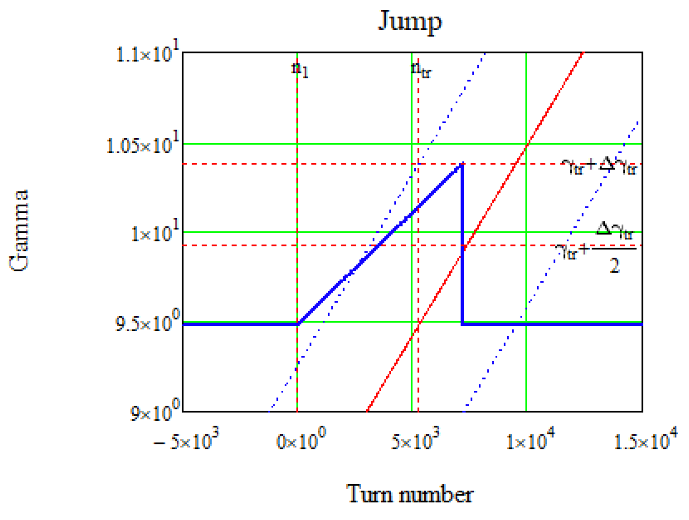
\includegraphics[width=1\columnwidth]{images/3_gamma_transition_jump_U70.png}
			\end{minipage}}
		\end{column}
		\begin{column}{0.4\textwidth}
			\begin{minipage}{\linewidth}
				\centering
				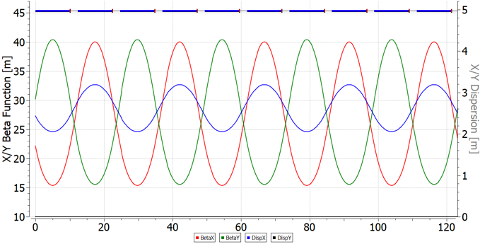
\includegraphics[width=1\columnwidth]{images/3_twiss_U70_regular.png}
				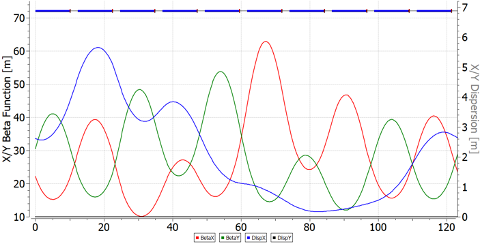
\includegraphics[width=1\columnwidth]{images/3_twiss_U70_modulated.png}
			\end{minipage}
		\end{column}
	\end{columns}
\end{frame}
%------------------------------------------------
\begin{frame}
	\frametitle{Данные с сеанса на У-70}
	\centering
	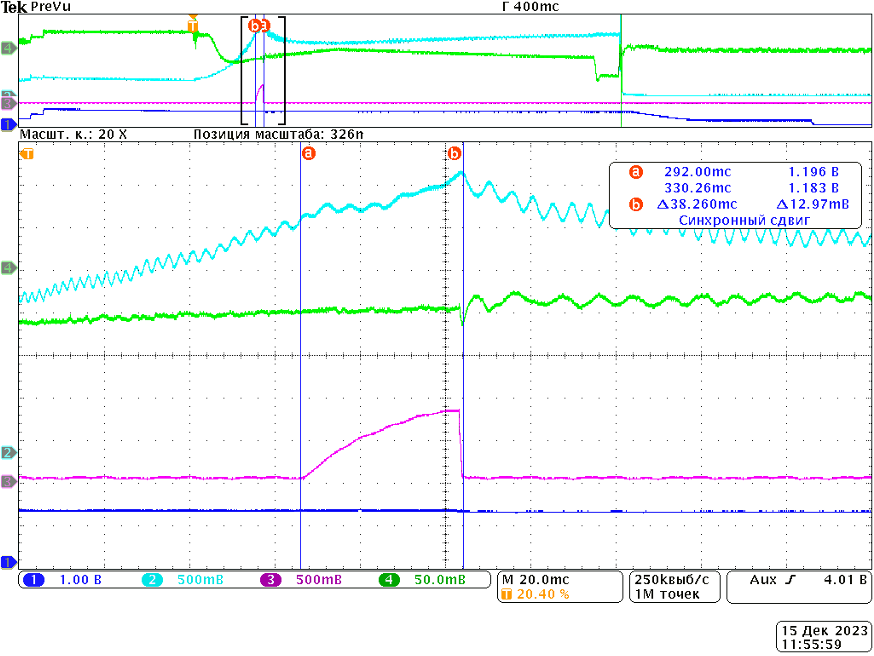
\includegraphics[width=0.30\columnwidth]{3_jump_U70_oscilogram.png}
	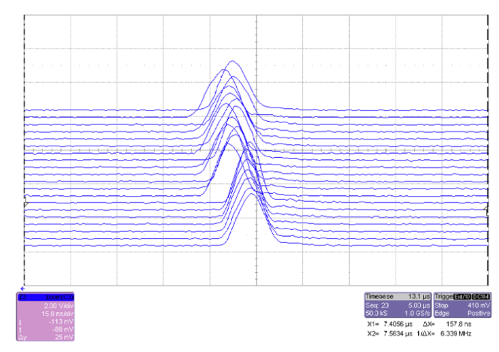
\includegraphics[width=0.323\columnwidth]{3_jump_U70_beam_profile.png}
	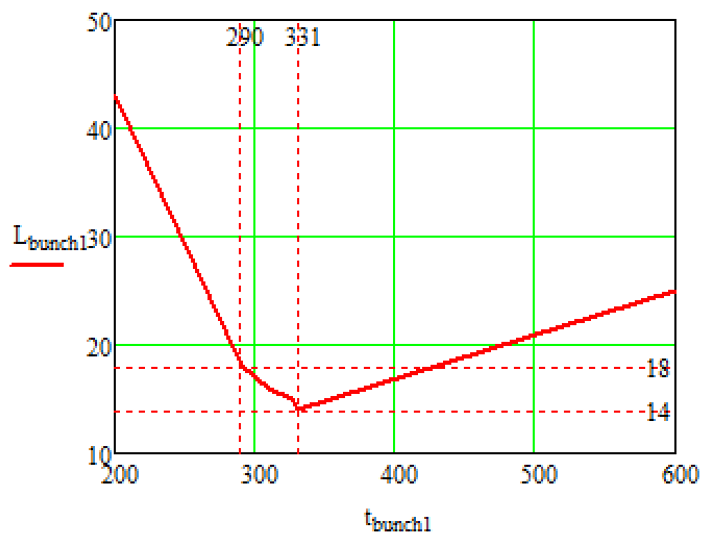
\includegraphics[width=0.30\columnwidth]{3_jump_U70_beam_lenght.png}
\footnotetext[4]{Kolokolchikov, S.D., Senichev, Y.V. \& Kalinin, V.A. Transition Energy Crossing in Harmonic RF at Proton Synchrotron U-70. Phys. Atom. Nuclei 87, 1355–1362 (2024). https://doi.org/10.1134/S106377882410020X}
\end{frame}
%------------------------------------------------
\begin{frame}
	\frametitle{Скачок критической энергии в NICA}
	
	Для NICA $\Delta\gamma_{\textrm{tr}}=1.1\Delta q$. Максимальная вариация частоты или рабочей точки составляет $\pm\Delta q=0.05$, что соответствует измерению критической энергии порядка $\Delta\gamma_{\textrm{tr}}=0.09$
	
	\centering
	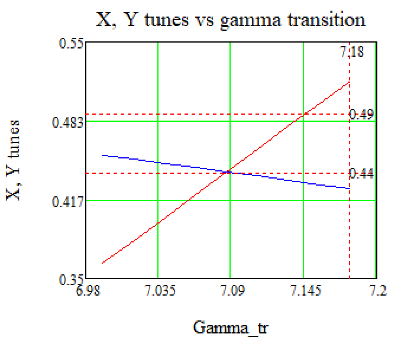
\includegraphics[width=0.35\columnwidth]{3_tunes_vs_g_tr.png}
	\includegraphics[width=0.35\linewidth]{3_Jump_NICA}
\footnotetext[5]{Kolokolchikov S.D. et al. Transition Energy Crossing in NICA Collider of Polarized Proton Beam in Harmonic and Barrier RF. Phys. Atom. Nuclei 87, 1449–1454 (2024). DOI: 10.1134/S1063778824100211}
\end{frame}
%------------------------------------------------
\begin{frame}
	\frametitle{Скачок критической энергии в барьерном ВЧ}
	\centering
	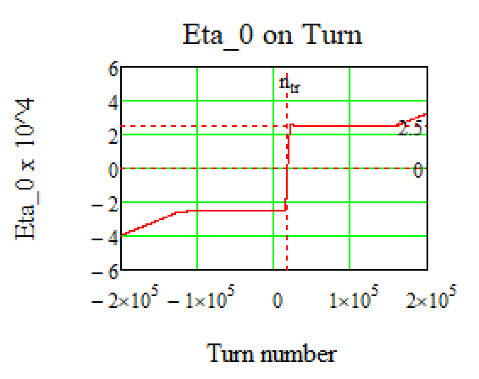
\includegraphics[width=0.4\columnwidth]{3_eta_tr_BB.png}
	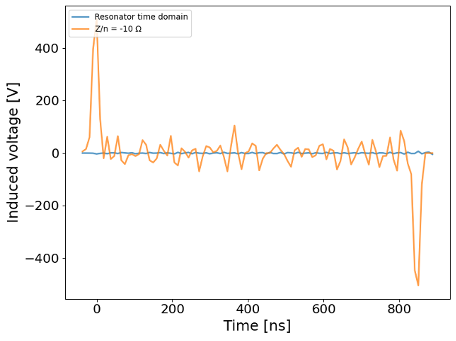
\includegraphics[width=.45\columnwidth]{3_induced_voltage}
\footnotetext[6]{Kolokolchikov S. et al. Longitudinal Dynamic in NICA Barrier Bucket RF System at Transition Energy Including Impedances in BLonD. Phys. Part. Nuclei Lett. 21, 419–424 (2024). DOI: 10.1134/S1547477124700389}
\footnotetext[7] {Kolokolchikov S., Acceleration and crossing of transition energy investigation using an RF structure of the barrier bucket type in the NICA accelerator complex. J.Phys.Conf.Ser. Vol. 2420, 012001 (2023). DOI: 10.1088/1742-6596/2420/1/012001}
\end{frame}
%------------------------------------------------
\begin{frame}
	\frametitle{Продольная микроволновая неустойчивость}
	\begin{equation}
		N_p\le K_1K_2\frac{E_0}{\left(\left|Z_\parallel\right|/n\right)ec}\left|\eta\right|\gamma\beta\sigma_p^2L_{\textrm{B}};
		\quad \quad
		N_p\le K_1K_2\frac{E_0}{\left(\left|Z_\parallel\right|/n\right)ec}\left|\eta\right|\frac{4\varepsilon_{\text{tr}}^2}{{\pi\gamma\beta L}_{\textrm{B}}}
		\label{eq:microwave_instability_2}
	\end{equation}
	\centering
	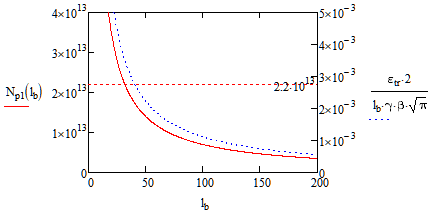
\includegraphics[width=0.6\columnwidth]{3_microwave_inst_vs_lenght.png}
\end{frame}
%------------------------------------------------
%------------------------THIRD------------------------
%------------------------------------------------
\section{Исследование ЭДМ}
%------------------------------------------------
\begin{frame}
	\centering \Large{Исследование ЭДМ}
\end{frame}
%------------------------------------------------
\begin{frame}
	\frametitle{Т-БМТ уравнение эволюции спина}
	\par В случае измерения ЭДМ заряженных частиц необходимо использование ускорителя заряженных частиц
	\par Т-БМТ уравнение описывает эволюцию поведения спина во внешних полях
	
	\begin{equation}	
		\begin{aligned} 
			\dv{{\vec{S}}}{t} &=\left(\vec{\Omega}_{\textrm{MDM}}+\vec{\Omega}_{\textrm{EDM}}\right) \times \vec{S}, \\
			\vec{\Omega}_{\textrm{MDM}}&=-\frac{q}{m \gamma}\left\{(\gamma G+1)\vec{B}_{\perp}+(G+1)\vec{B}_{\parallel}-\left(\gamma G+\frac{\gamma}{\gamma+1}\right) \frac{\vec{\beta} \times \vec{E}}{c}\right\}, \\
			\vec{\Omega}_{\textrm{EDM}}&=-\frac{q \eta}{2 m}\left(\vec{\beta} \times \vec{B}+\frac{\vec{E}}{c}-\frac{\gamma}{\gamma+1}\frac{\vec{\beta}}{c}\left(\vec{\beta}\cdot\vec{E}\right)\right), \quad G=\frac{g-2}{2}
		\end{aligned}
		\label{eq:T-BMT}
	\end{equation}
\end{frame}
%------------------------------------------------
\begin{frame}
	\frametitle{Квази-замороженный спин}
	Условия квази-замороженного спина
	\begin{equation}
		\tiny
		\Phi_p^{\textrm{arc}}+\Phi_{p}^{\textrm{comp}}=\frac{2\pi}{N};\quad \Phi_s^{\textrm{arc}}+\Phi_{s}^{\textrm{comp}}=0
		\label{eq:QFS_orbital}
	\end{equation}
	\normalsize
	Длина компенсирующего элемента
	\begin{equation}
		\tiny
		L_{\text{min}} = \Phi_{p\mathrm{E}}^{\text{comp}}R_{\mathrm{E}}=
		\frac{2\pi}{N}\frac{\gamma^2 G}{G+1}\frac{\kappa}{\mathrm{E}_{\text{max}}}
		= \frac{2\pi}{N}\frac{G}{G+1}\frac{mc^2}{e}\frac{\gamma(\gamma^2-1)}{\mathrm{E}_{\text{max}}}.
		\label{eq:length_min}
	\end{equation}
	\normalsize
	\centering
	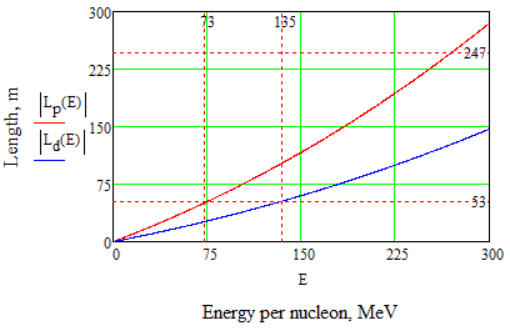
\includegraphics[width=0.3\columnwidth]{4_total_length}
\footnotetext[9]{(to be published) Kolokolchikov S.D., et al. Quasi-frozen spin for both deuteron and proton beam at periodic EDM storage ring lattice, Nucl.Sci. and Tech.}
\end{frame}
%------------------------------------------------
\begin{frame}
	\frametitle{Электростатический дефлектор}
	\centering
	а. Дейтрон\quad\quad\quad\quad\quad\quad\quad\quad\quad\quad\quad\quad\quad\quad\quad б. Протон \\
	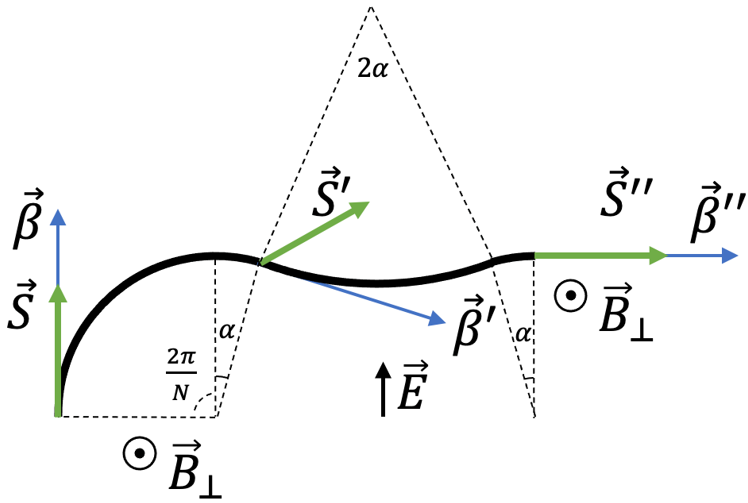
\includegraphics[width=0.4\columnwidth]{4_deflector_deutron}
	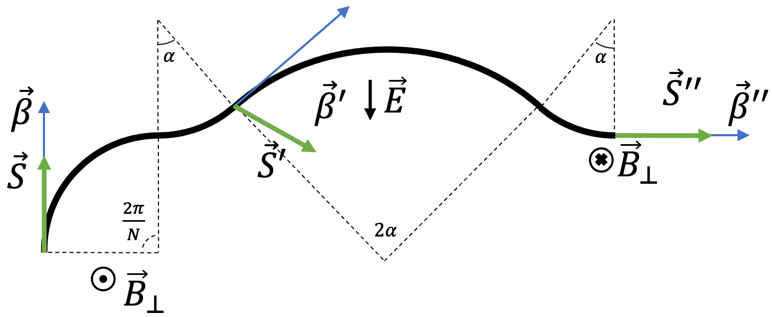
\includegraphics[width=0.5\linewidth]{4_deflector_proton}
\end{frame}
%------------------------------------------------
%------------------------------------------------
\begin{frame}
	\frametitle{Фильтр Вина}
	\centering
	а. Дейтрон\quad\quad\quad\quad\quad\quad\quad\quad\quad\quad\quad\quad\quad\quad\quad\quad б. Протон \\
	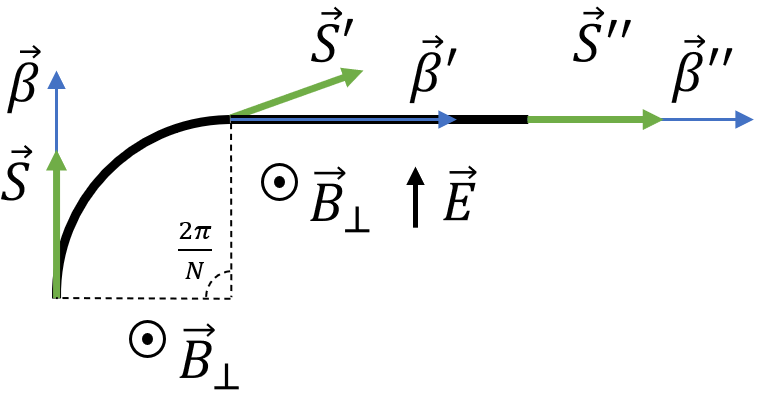
\includegraphics[width=0.49\linewidth]{4_wien-filter_deuteron}
	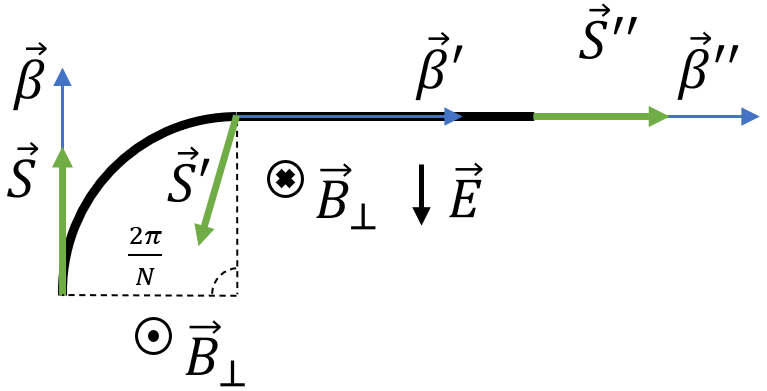
\includegraphics[width=0.49\linewidth]{4_wien-filter_proton}
\end{frame}
%------------------------------------------------
\begin{frame}
	\frametitle{Модернизация Nuclotron 16-ти периодическая структура}
		\begin{columns}
		\begin{column}{0.5\textwidth}
			\raggedright
			\adjustbox{valign=t}{\begin{minipage}[t]{\linewidth}
				Отличие измерения ЭДМ в квази-замороженной и замороженного структуре, в первом порядке
				\begin{equation}
					J_{0}(\Phi_s^{\textrm{arc}})=1-\frac{{\Phi_s^{\textrm{arc}}}^2}{4},
					\label{eq:edm}
				\end{equation}
			\end{minipage}}
		\end{column}
		\begin{column}{0.5\textwidth}
			\begin{minipage}{\linewidth}
				\centering
				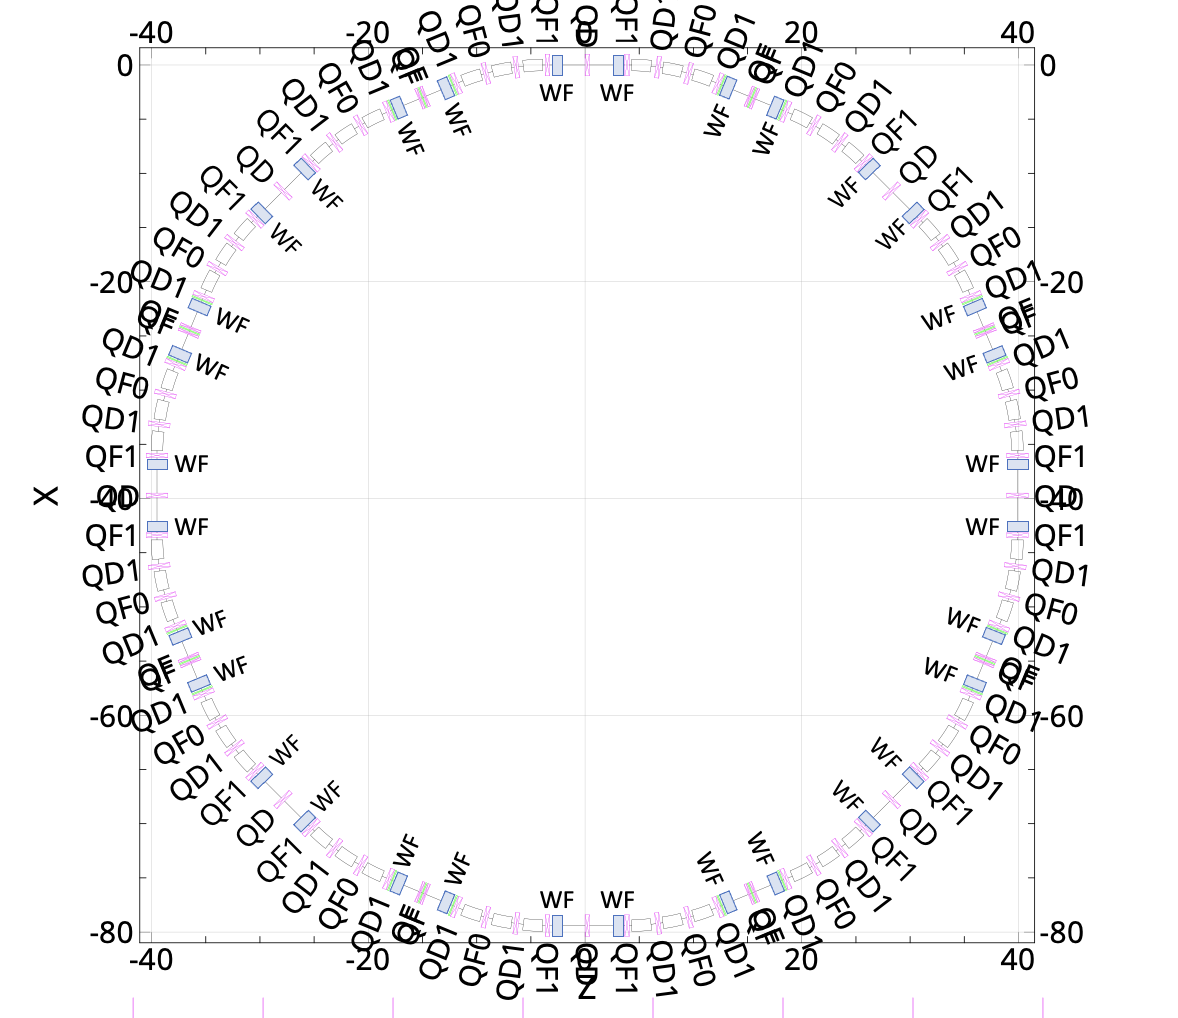
\includegraphics[width=0.9\columnwidth]{4_Nuclotron_16.png}
			\end{minipage}
		\end{column}
	\end{columns}
\end{frame}
%------------------------------------------------
\begin{frame}
	\frametitle{NICA bypass}
	\centering
	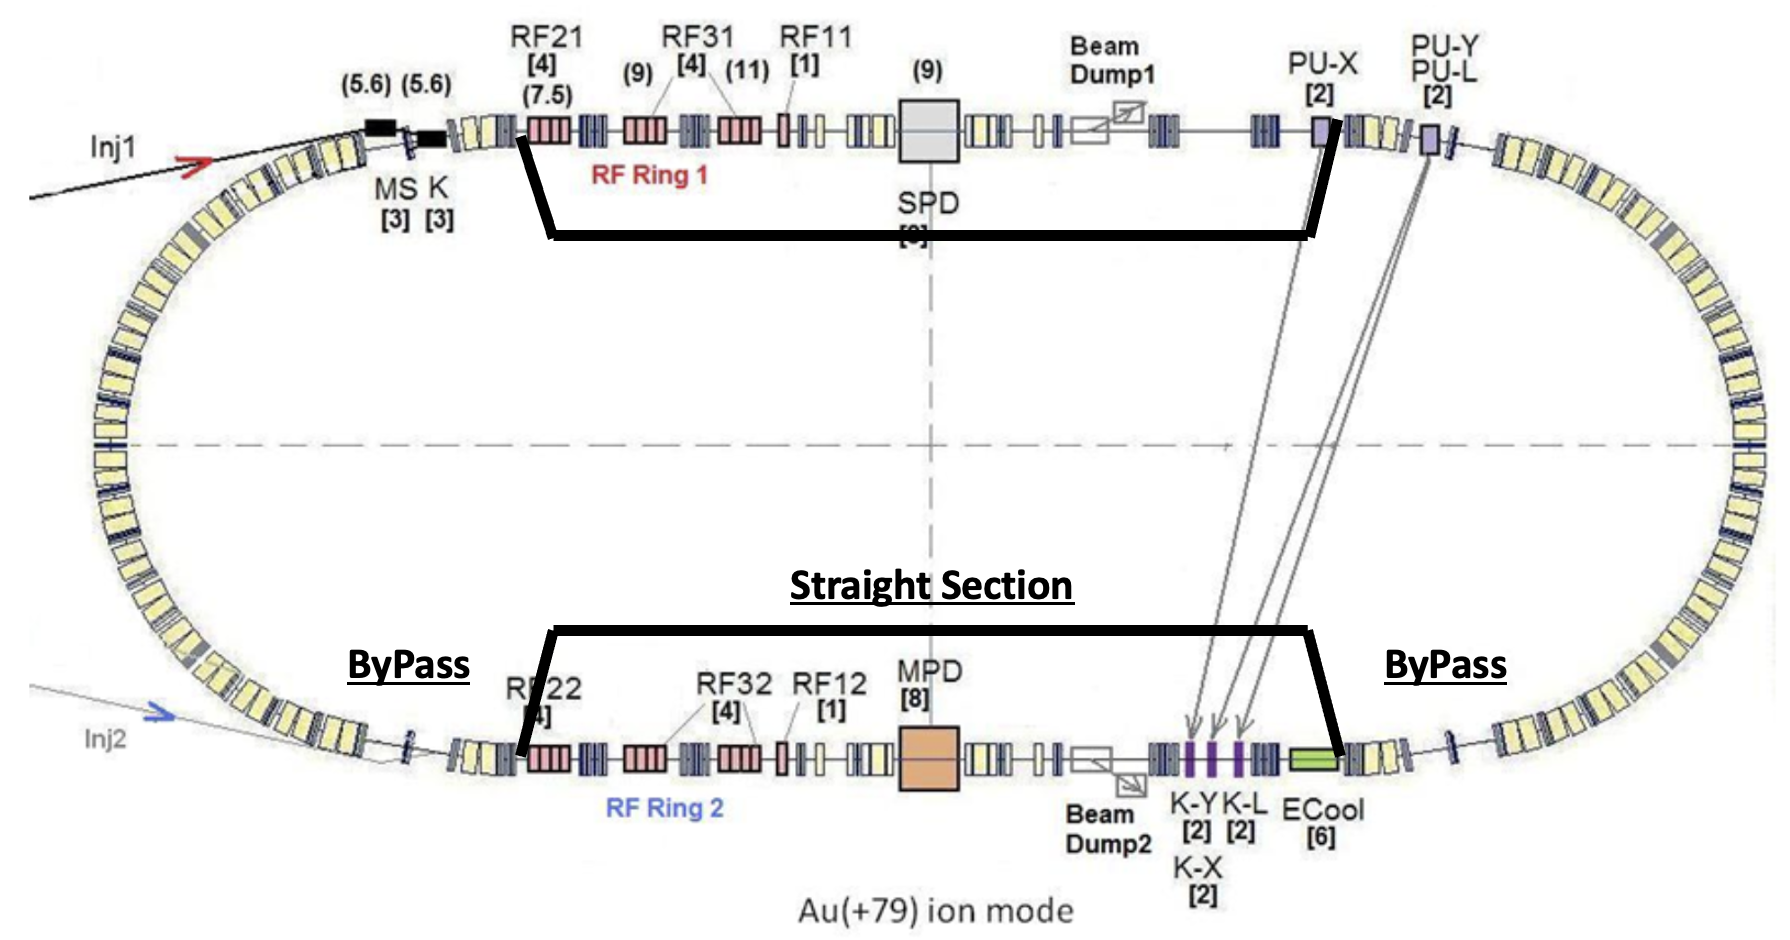
\includegraphics[width=0.65\columnwidth]{4_NICA_bypass.png}
\footnotetext[10]{Колокольчиков С.Д. и др. Проектирование Каналов Bypass в Ускорительном Комплексе NICA для Экспериментов с Поляризованными Пучками по Поиску ЭДМ. Яд. Физ. и Инж. том 15, номер 5, стр. 457-463 (2024). DOI: 10.56304/S2079562924050257}
\footnotetext[11]{S. Kolokolchikov et al. ByPass optics design in NICA storage ring for experiment with polarized beams for EDM search. J.Phys.Conf.Ser. Vol. 2687, 022026 (2024). DOI: 10.1088/1742-6596/2687/2/022026}
\end{frame}
%------------------------------------------------
\begin{frame}
	\frametitle{Декогеренция спина}
	\centering
	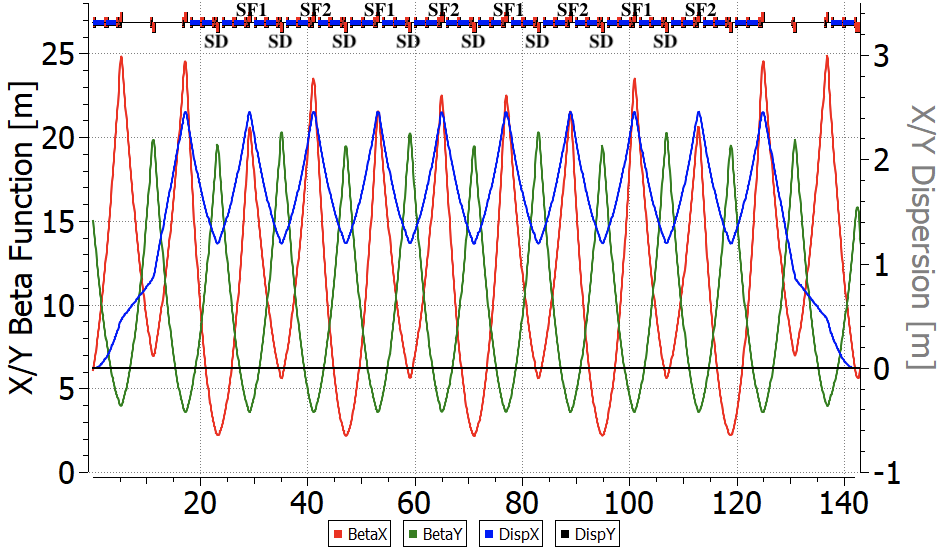
\includegraphics[width=0.55\columnwidth]{4_NICA_arc.png}
	\footnotetext[12]{Kolokolchikov S. et al. Spin Coherence and Betatron Chromaticity of Deuteron Beam in “Quasi-Frozen” Spin Regime. Phys. Atom. Nuclei 86, 2684–2688 (2023). DOI: 10.1134/S106377882311025X}
	\footnotetext[13]{S. Kolokolchikov et al. Spin coherence and betatron chromaticity of deuteron beam in NICA storage ring. J.Phys.Conf.Ser. Vol. 2687, 022027 (2024). DOI: 10.1088/1742-6596/2687/2/022027}
\end{frame}
%------------------------------------------------